%\documentclass[12pt,twocolumn]{article}
\documentclass[12pt]{article}
\usepackage[utf8]{inputenc}
\usepackage{amsmath}
\usepackage{listings}
\usepackage{graphicx}
\title{A Genetic Program for Symbolic Regression \\
CS 472 Fall 2011 \\
     Project 2}
\author{Colby Blair}
\date{Due October 26th, 2011}

\begin{document}
\maketitle

\begin{abstract}
In computer science, one area of study is that of optimization. Genetic Algorithms (GAs) optimize functions, while Genetic Programming (GP) tries to find functions to fit data. Genetic Programming creates mathematical expression trees, and are useful for finding the functions that are not known, given some data.

This report presents a GP with mathematical non-terminal symbols '+', '-', '*', and '/', and terminal values as contants and variables. This report demonstrates a GP for a very limited domain, and a few different target equations. It talks about the crossover and selection functions, as well as the population representation. This report uses a generational algorithm for population regeneration. This report demonstrates good results for the limited test set, and suggests improvements for the bad results. Finally, this report shows the code used.
\end{abstract}

\pagebreak

\tableofcontents

\pagebreak

\listoffigures

\pagebreak


\part{Introdution}
GPs are used to try to approximate a mathamatical expression \textbf{tree} (Section \ref{sec:trees}) that describes a function on a graph. In order to improve the approximation, a random set of expression trees are first randomly generated. This set is called the \textbf{population} (Section \ref{sec:population}). When trees are evaluated, they are measured by computing what each mathamatical expression's result is. The fitness is then the error rate, or $ value expected - value computed $. A \textbf{minimum fitness} in this report is, then, the best fitness in the population, and the max is the worst. Inverse to one's first inclination, but an abstract representation nonetheless.

Individuals in the population are then selected, crossed over (or bred together), and then mutated. Exactly how depends on the \textbf{random tree generator}, \textbf{selection}, \textbf{crossover}, \textbf{mutation} functions, and in the \textbf{generational algorithm}, which are described in Sections \ref{sec:rand_tree}, \ref{sec:selection}, \ref{sec:crossover}, \ref{sec:mutation}, and \ref{sec:gen_alg}, respectively.

\part{Experimentation}

\section{Representation Description}
\subsection{Trees}
\label{sec:trees}
\begin{figure}[!h]
        \begin{center}
		\scriptsize
		\begin{lstlisting}
	+---------------+
	|tree		|
	|tree_node *tnp=|------------------------------ +---------------+
	|...		|				|tree_node	|
	|int nchildren= |				|enum node_type	|
	| 2 (nonterminal)|				|double dval	|
	|tree *children[]|------			|double variable*|
	+---------------+	|			+---------------+
				|
				... (many more non-terminals)
		----------------|
		|		|
		|	+---------------+
		|	|tree		|
		|	|tree_node *tnp=|-------------- +---------------+
		|	|...		|		|tree_node	|
		|	|int nchildren= |		|enum node_type	|
		|	| 0 (terminal)	|		|double dval	|
		|	|tree *children[]|--NULL	|double variable*|
		|	+---------------+		+---------------+
	+---------------+
	|tree		|
	|tree_node *tnp=|------------------------------ +---------------+
	|...		|				|tree_node	|
	|int nchildren= |				|enum node_type	|
	| 0 (terminal)	|				|double dval	|
	|tree *children[]|-------NULL			|double variable*|
	+---------------+				+---------------+
		\end{lstlisting}
		\normalsize
               \caption{An expression tree (one per individual)}
                \label{tree_rep}
        \end{center}
\end{figure}

A tree is simply class, that has pointers to child trees. Since our operators ('+', '-', '*', and '/') only take a left hand and right hand expressions, each tree only needs at most \textbf{2 children}. But more or less can be inserted for future operators, on a per-operator basis. The '/' division operator is protected by \textbf{division by zero} errors by simply returning a 0 result if any denominator is 0. Since a tree simply points to other subtrees, the term \textbf{tree} in this report can mean either the whole tree or a subtree.

Our operators are called \textbf{non-terminals}, since they rely on the results of child subtrees to compute their results. Our \textbf{terminals} then are either constants or pointers to elements in a variable array (double, or decimal, values). Both are initialized randomly from their respective sets. The variable array can be of \textbf{any practical size} (${x_1, x_2, ... x_n}$).

Each tree class instance points to a tree\_node class. This class holds the enumerable type of the tree class; either 'plus', 'minus', 'multi', or 'div' for non-terminal trees (operators), or 'tree\_double' or 'tree\_variable' for terminal trees.

The terminal (tree) nodes are mutated using point mutation 90\% of the time. 10\% of the time, the non-terminal trees are mutated by simple regenerating a random tree in place, and selected at random. Trees of type tree\_var are, again, pointers to a variable array. This tree's value is initialized to point to a random element in the variable list. Since they are pointers, modifying variable values takes immediate affect throughout the tree. The variables in the variable array can be modified, and the tree evaluation and fitness functions (re)ran.

During the experiment, \textbf{depth issues} became a problem. Tree expanded hugely to protect themselves from destructive changes \cite{growth}, and tree evaluations hung due to huge tree search times. This report's approach is to simply limit the max tree depth result that a \textbf{crossover} or \textbf{mutation} would have. If a crossover or mutation would result in a tree max depth greater than a global max depth (12-14), the operation was aborted before it happened, and the tree's state was left alone.

\subsection{Population}
\label{sec:population}
In order to optimize lots of trees to reach an approximate solution, a \textbf{population} (or set) is kept. Our population is just a list (or array) of trees. 

\begin{figure}[!h]
        \begin{center}
		\begin{tabular}{r l}
	                $ P = i_1, i_2, ... i_j $	& \\
								& where \\
								& $ i_n $ is a tree\\
								& $ j = 500 $ \\
		\end{tabular} 
               \caption{The representation of the population}
                \label{population}
        \end{center}
\end{figure}


\section{Functions and Generators}
\subsection{Fitness Function}
\label{sec:fitness}
\begin{figure}[!h]
        \begin{center}
		\begin{tabular}{r l}
			$ f_i(expected) $		&	$ = $ Error \\
								&	$ = | eval_i() - expected | $ \\
								& where \\
								& $ eval_i() $ is the evaluation function in Figure \ref{eval_func}\\
		\end{tabular}
               \caption{Fitness function}
                \label{fit_func}
        \end{center}
\end{figure}

The $fitness_i()$ and $eval_i()$ functions only ever consider one set of values for variables in the variable array for an optimization. For example, for each generation, $x_1 = .2, x_2 = .3$. The GP would then find a fairly good equation for these values. But not a very good solution for others. This is admitted a weak point in the experiment, and could be improved by running simulations again with an optimized population, and new variable values. An evaluation could also consider multiple value sets for each variable. Due to develop and compute time restraints, this was not improved, but would be fairly simple to do.

\begin{figure}[!h]
        \begin{center}
		\begin{tabular}{r l}
			$ eval_i() $	&	$ = \sum_{x=1}^{n} eval_{child_x}() $	if $i$ type is 'plus'\\
						&	$ = eval_{child_1}() - eval_{child_2}() - ... eval_{child_n}()$ if $i$ type is 'minus'\\
						&	$ = \prod_{x=1}^{n} eval_{child_x} $	if $i$ type is 'plus'\\
						&	$ = eval_{child_1}() / eval_{child_2}() / ... eval_{child_n}()$ if $i$ type is 'div'\\
						&	$ = i_{constant value} $ if $i$ type is 'tree\_double' \\
						&	$ = i_{variable valu} $ if $i$ type is 'tree\_var' \\
						& where \\
						& $ n $ is the number of children (0 or 2 only for now)
		\end{tabular}
               \caption{Evaluation function}
                \label{eval_func}
        \end{center}
\end{figure}

\subsection{Random Tree Generator}
\label{sec:rand_tree}
\begin{figure}[!h]
        \begin{center}
		\scriptsize
		\begin{lstlisting}
if random_value in 0...9 equals 0 or at depth 0:
	set this subtree to a terminal type; a randomly a contant or 
		a variable
else:
	set this subtree to a nonterminal type; randomly a 'plus', 
		'minus','multi','div'
	create each child from rand_tree_generator(depth - 1)
		\end{lstlisting}
		\normalsize
               \caption{Random tree generator}
                \label{rand_tree_gen}
        \end{center}
\end{figure}

\subsection{Select Function}
\label{sec:selection}
\begin{figure}[!h]
        \begin{center}
		\begin{tabular}{r l}
			$ selection(P) = $		&	$ i_1, i_2, ... i_j$ \\
								& \\
								&	where \\
								&	$ P $ is the entire population \\
								&	$ i_j $ is a random individual \\
								&	$ k $ is the sample size, specified at run time (default = population size / 10, or 10\%) \\
		\end{tabular} 
               \caption{The selection function}
                \label{selection_future}
        \end{center}
\end{figure}

Note that a higher $ k $ value will find local minimum fitnesses (best fitnesses) faster, while a lower $ k $ will leave more variance in the population, because the minimum (best) fitnesses are less likely to reproduce. 

\subsection{Crossover Function}
\label{sec:crossover}
\begin{figure}[!h]
        \begin{center}
		\begin{lstlisting}
MAX_DEPTH = 12...14 #depending on simulation
for original tree1:
	select random tree 1 nonterminal
	select random tree 2 nonterminal
	if tree 1 max depth (including random tree 2 nonterminal) 
		< MAX_DEPTH:
			replace it with random tree 2 nonterminal
	else:
		ignore
for original tree2:
	select random tree 1 nonterminal
	select random tree 2 nonterminal
	if tree 2 max depth (including random tree 1 nonterminal) 
		< MAX_DEPTH:
			replace it with random tree 1 nonterminal
	else:
		ignore
		\end{lstlisting}
               \caption{Crossover function (see Section \ref{sec:tree.cpp})}
                \label{fit_func}
        \end{center}
\end{figure}

\pagebreak

\subsection{Mutation Function}
\label{sec:mutation}
\begin{figure}[!h]
        \begin{center}
		\scriptsize
		\begin{lstlisting}
for i in random 1..10
if i == 1:
	#regenerate subtree
	for j in rand 1..number of nonterminal nodes in the tree:
		nonterm tree node j = random_gen_nonterm
		return
else:
	#point mutation
	for i in rand 1..number of terminal nodes in the tree:
		term tree node j = rand_gen_term
		return
		\end{lstlisting}
		\normalsize
               \caption{The mutation function}
                \label{mut_func}
        \end{center}
\end{figure}

\subsection{Generational Algorithm}
\label{sec:gen_alg}
\begin{figure}[!h]
        \begin{center}
		\scriptsize
		\begin{lstlisting}
while not bored:
	select k random individuals using selection function
	select the 2 best (tournament selection) as parents, and crossover using
		the crossover function
	for each of the individuals in the population:
		take the best of the 2 parents, and mutate slightly as new mutatant child
		replace individual with new mutant child

	if minimum fitness <= .0001 or 1000 generations:
		bored = true
		\end{lstlisting}
		\normalsize
               \caption{The generational algorithm}
                \label{gen_alg}
        \end{center}
\end{figure}


\pagebreak


\part{Results}
For the results, the equation $x^3 + 5y^3 - 4xy + 7$ is considered. For optimization, $ x = .2, y = .3$.  Below are the graphs and tables for the simulation and actual function.

\begin{figure}[!h]
        \begin{center}
		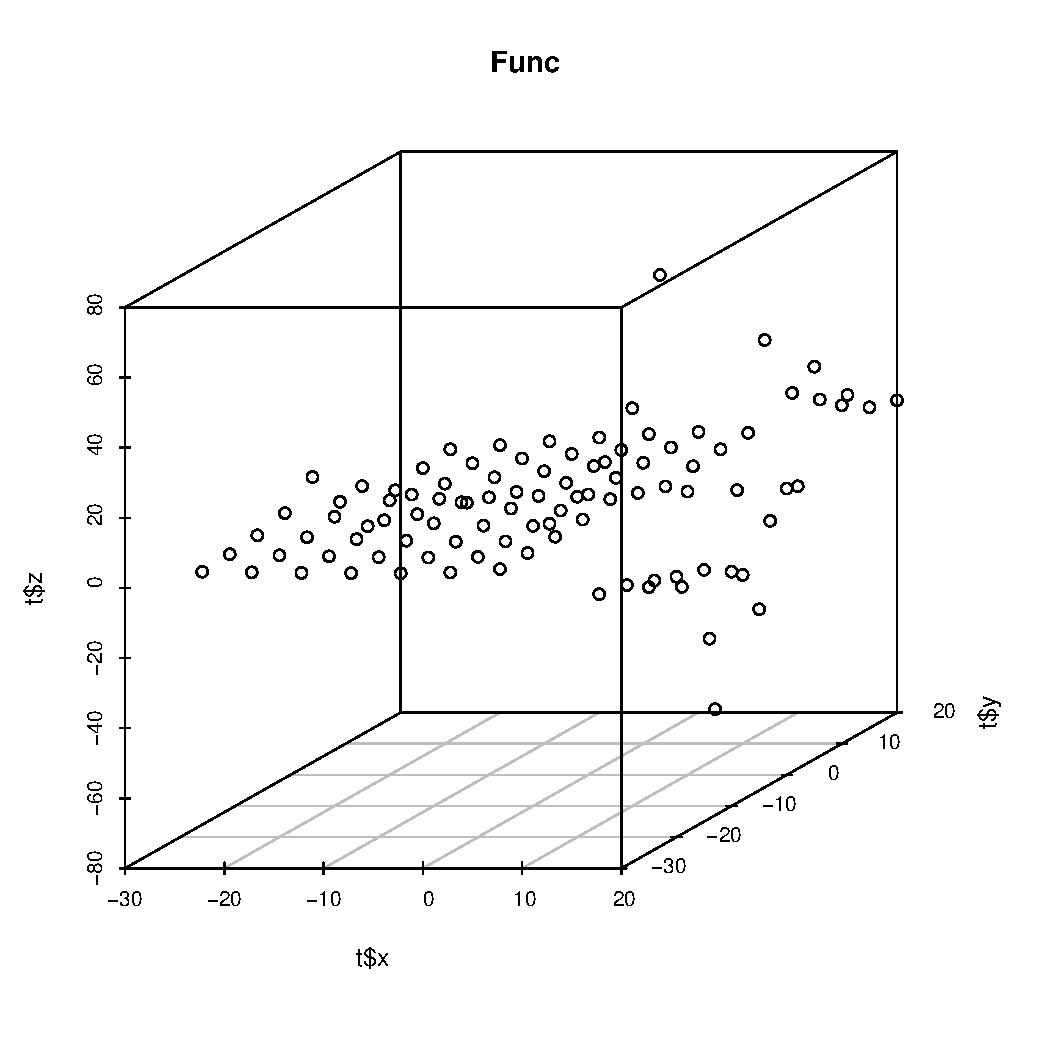
\includegraphics[width=70mm]{results.pdf}
               \caption{Our best individual results}
                \label{results}
        \end{center}
\end{figure}

\lstinputlisting{results.txt}

\begin{figure}[!h]
        \begin{center}
		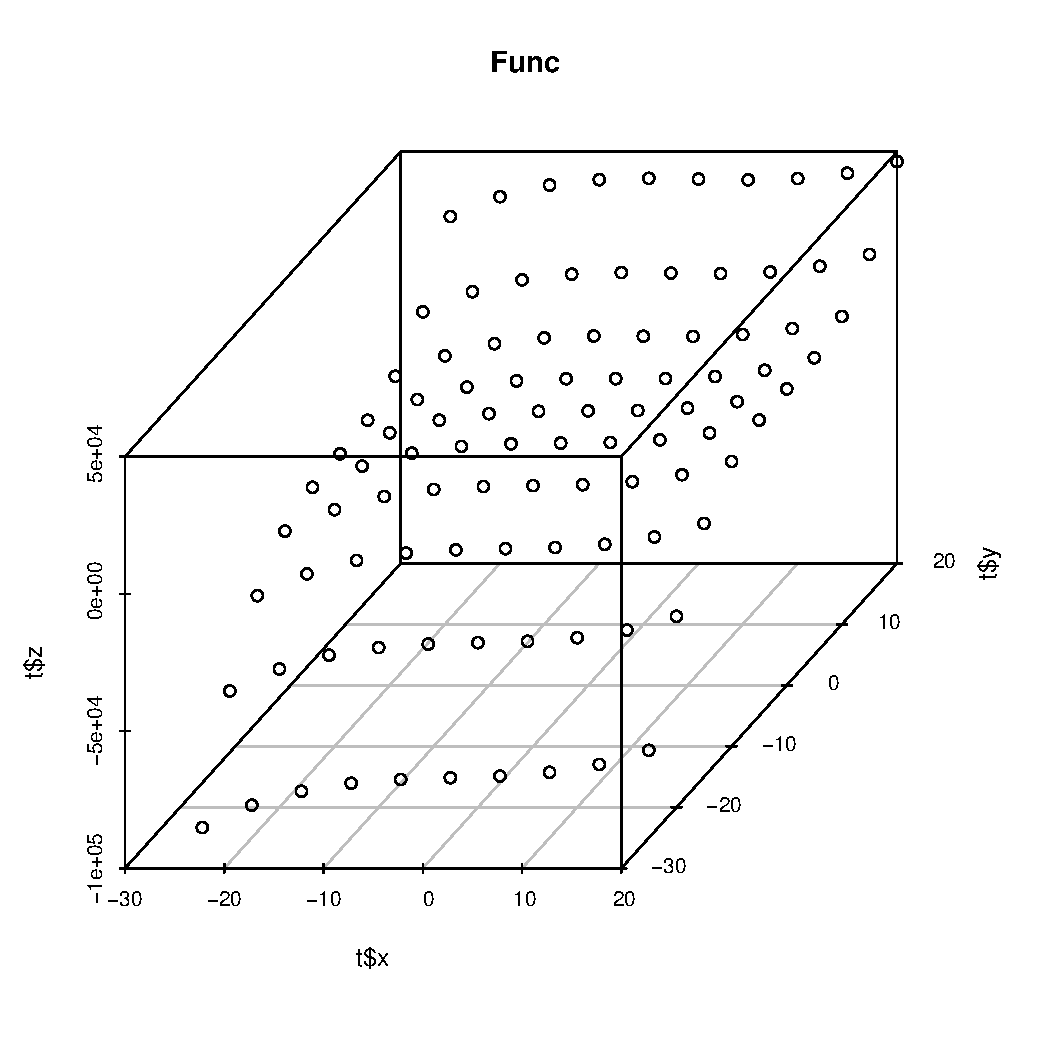
\includegraphics[width=70mm]{func.pdf}
               \caption{Actual function values}
                \label{results}
        \end{center}
\end{figure}

\lstinputlisting{func.txt}

\part{Conclusion}
In conclusion, the GP did great for $x = .2, y = .3$. But since it didn't consider any other values yet in optimization, the overall results were very bad. With a little more development and much more compute time, optimizing over all the values that this report graphed for the actual function would lead to a much better GP overall.

This report doesn't show overall good results. But it does show a reasonable approach to GPs and linear regression problems. Much more could be done with different population algorithms (steady state vs. generational), as well as with elitism vs. no elitism. More could be done also with different $k$ values in the selection function, and with more experimentation, better results would be achievable.

Tree growth in regard to depth was a constant concern in development. Trees tend to grow to hide entrons and minimize destructive mutations and crossovers\cite{growth}. To identify this problem, this report set MAX\_DEPTH to a low number, like 5. This lead to an opposite problem; minimum fitnesses were always depth 1 trees, or an expression like $ x * 15 $. The depth was not enough to statistically have good mutations/crossovers; most chagnes to depth 5 were very destuctive, and immediately destroyed. There seemed to be a sweet spot around MAX\_DEPTH = 9 before this problem went away. After that, most tree grew immediately to the MAX\_DEPTH, and had many intron branches.

Performance wise, this report used a lower level program language (C++) over interpretive langauges like R or Python. This lead to much higher development time, but much better tree evaluation time compared to our past experience. The performance time was nice, but GP's have an area for parallelism in tree evaluations that is perhaps nicer than GA's fitness evaluations. The deeper the tree, the better the solution, although with diminishing returns. Each tree evaluation is independent of another, so this problem lends itself well to true task parallellism.

\part{Bibliography}

\begin{thebibliography}{99}
\bibitem{growth} Harrison, M.L.; Foster, J.A. "Improving the Survivability of a Simple Evolved Circuit through Co-evolution". { \em  Evolvable Hardware, 2004. Proceedings. 2004 NASA/DoD Conferenc } 24-26 June 2004 : 123-129. Print

\end{thebibliography}


\pagebreak


%\part{Output}
%\section{A sample run}
%\lstinputlisting{sample_run1.txt}



\part{Code}
\footnotesize
\subsection{Makefile}
\lstinputlisting{src/Makefile}

\subsection{main.h}
\lstinputlisting{src/main.h}

\subsection{main.cpp}
\lstinputlisting{src/main.cpp}

\subsection{tree\_node.h}
\lstinputlisting{src/tree_node.h}

\subsection{tree\_node.cpp}
\lstinputlisting{src/tree_node.cpp}

\subsection{tree.h}
\lstinputlisting{src/tree.h}

\subsection{tree.cpp}
\label{sec:tree.cpp}
\lstinputlisting{src/tree.cpp}

\subsection{darray.h}
\lstinputlisting{src/darray.h}

\subsection{darray.cpp}
\lstinputlisting{src/darray.cpp}

\subsection{tree\_gp.h}
\lstinputlisting{src/tree_gp.h}

\subsection{tree\_gp.cpp}
\label{sec:tree-gp.cpp}
\lstinputlisting{src/tree_gp.cpp}

\subsection{test.h}
\lstinputlisting{src/test.h}

\subsection{test.cpp}
\lstinputlisting{src/test.cpp}


\end{document}
